\documentclass[../../main.tex]{subfiles}
\begin{document}
\setcounter{footnote}{0} 

\newcommand{\ade}{\emph{autodE }}

\NewDocumentCommand{\code}{v}{%
	\texttt{\textcolor{black}{#1}}%
}

\section{Further Developments}

Since its publication in late 2020, a number of developments have been introduced into \ade to enhance functionality and reduce computational expense. These are outlined in the following sections, with in-progress developments itemised on the online repository.\footnote{See \url{https://github.com/duartegroup/autodE/projects} for current developments.}

\subsection{Transition State Guesses}

The initial \ade implementation to generate TS guess geometries made use of relaxed 1D and 2D relaxed PES scans over the breaking/forming coordinates to search for a saddle point. This approach was employed based on the conventional human-guided method of calculating reaction profiles, but has some limitations: (1) a uniform step is taken, meaning the computational effort cannot be focused around the saddle point; (2) for high energy unphysical reactions involving two active bonds 1D low-level, 1D high-level, 2D low-level and 2D high-level searches were employed in sequence only to perhaps not find a TS; (3) 2D high-level surfaces are expensive to compute, thus for e.g. a Diels-Alder reaction where a low GFN2-XTB method is insufficiently accurate, 64 DFT optimisations were required. Therefore, a nudged elastic band (NEB)\cite{NEB1998} along with its climbing image variant (CI-NEB)\cite{Henkelman2000CINEB} were implemented as follows. The energy of a number of structures (`images') along a path are minimised under a force $\boldsymbol{F}$. Specifically, the implementation follows that of Henkelman\cite{Henkelman2000NEB} where, for an image $i$ in the nudged elastic band,
\begin{equation}
	\boldsymbol{\tau}_i = 
	\begin{cases}
		\boldsymbol{\tau}_i^+ &\quad\text{if}\quad V_{i-1} < V_i < V_{i+1} \\
		\boldsymbol{\tau}_i^- &\quad\text{if}\quad V_{i+1} < V_i < V_{i-1} \\
		\boldsymbol{\tau}_i^+\Delta V_i^{max} + \boldsymbol{\tau}_i^-\Delta V_i^{min} &\quad\text{if}\quad V_{i-1} <  V_{i+1} \\
		\boldsymbol{\tau}_i^+\Delta V_i^{min} + \boldsymbol{\tau}_i^-\Delta V_i^{max} &\quad\text{if}\quad V_{i+1} < V_{i-1} \\
	\end{cases}
\end{equation}
where,
\begin{equation}
	\begin{aligned}
		\boldsymbol{\tau}_i^+ &= \boldsymbol{R}_{i+1} - \boldsymbol{R}_i \\
		\boldsymbol{\tau}_i^- &= \boldsymbol{R}_{i} - \boldsymbol{R}_{i-1}
	\end{aligned}
\end{equation}
and,
\begin{equation}
	\begin{aligned}
		\Delta V_i^{max} &= \max(|V_{i+1} - V_i|, |V_{i-1} - V_i|) \\
		\Delta V_i^{min} &= \min(|V_{i+1} - V_i|, |V_{i-1} - V_i|)
	\end{aligned}
\end{equation}
and $\boldsymbol{R}_i$ are the coordinates of image $i$. The spring force is,
\begin{equation}
	\boldsymbol{F}^s_i|_{\parallel} = (k_i|\boldsymbol{R}_{i+1} - \boldsymbol{R}_i| - k_{i-1}|\boldsymbol{R}_i - \boldsymbol{R}_{i-1}|) \hat{\boldsymbol{\tau}}_i
\end{equation}
and the total force on the image,
\begin{equation}
	\boldsymbol{F}_i = \boldsymbol{F}^s_i|_{\parallel} - \nabla V(\boldsymbol{R}_i)|_\perp
\end{equation}
where,
\begin{equation}
	\nabla V(\boldsymbol{R}_i)|_\perp = \nabla V(\boldsymbol{R}_i) - \nabla V(\boldsymbol{R}_i)\cdot \hat{\boldsymbol{\tau}}_i\hat{\boldsymbol{\tau}}_i
\end{equation}
and finally $\hat{\boldsymbol{\tau}} = \boldsymbol{\tau}_i/|\boldsymbol{\tau}_i|$.
\\
The climbing image (CI) NEB implementation follows that in ref. \cite{Henkelman2000CINEB}, where after a few iterations the force on the maximum energy image ($m$) is given by,
\begin{equation}
	\boldsymbol{F}_{m} = -\nabla V(\boldsymbol{R}_m) + 2\nabla V(\boldsymbol{R}_m)\cdot \hat{\boldsymbol{\tau}}_i\hat{\boldsymbol{\tau}}_i
\end{equation}
which is the force due to the potential along the band being inverted.

Employing a NEB relaxation of a path and taking the highest lying point on the approximate minimum energy pathway (MEP) as a transition state guess, however, relies on an initial reasonable path to relax along, and the NEB not corner cutting (i.e. the images relaxing into the reactant/product basins). To develop an initial path reactant and product complexes were overlapped and interpolation in Cartesian coordinates was employed. It is, however, challenging to align and rotate dihedrals to minimise the difference. Instead, a linear path from reactants to products over the changing bond lengths (i.e. sequential constrained minimisations) was an improvement but can lead to unexpected dissociations.\footnote{For example, the E2 elimination using methoxide+propyl chloride on a linear path using GFN2-XTB generates an unphysical [H$_3$CCHCH$_3$]+ cation.} In an attempt to reduce corner cutting an adaptive force constant, where $k$ is larger at images with higher energy, was introduced and is, generally  efficient.\cite{Henkelman2000NEB}
\begin{equation}
	k_m = 
	%\begin{cases}
		k_\text{max} - \Delta k \left(\frac{V_\text{max} - V_m}{V_\text{max} - V_\text{ref}} \right) \quad \text{if}\quad V_m > V_\text{ref} \qquad\text{  else  }\quad
		k_m = k_\text{min}  % \qquad\qquad\qquad\qquad\quad\;\;  
%	\end{cases}
\label{equation::neb_adaptive_k}
\end{equation}
where $V_\text{ref} = \max(V_n, V_0)$ and $\Delta k = k_\text{max} - k_\text{min}$.

For example, for a 1,2-shift in a terminal propyl radical using a fixed force constant and relaxing the NEB leads to two images very close to the fixed end points while the two higher lying images cut the barrier peak and miss a close TS geometry (\figurename{ \ref{fig::ade_further_1}}). Although improved using an adaptive force constant, this effect is one reason why NEB relaxation is not employed by default in \emph{autodE}.

\begin{figure}[h!]
	\vspace{0.4cm}
	\centering
	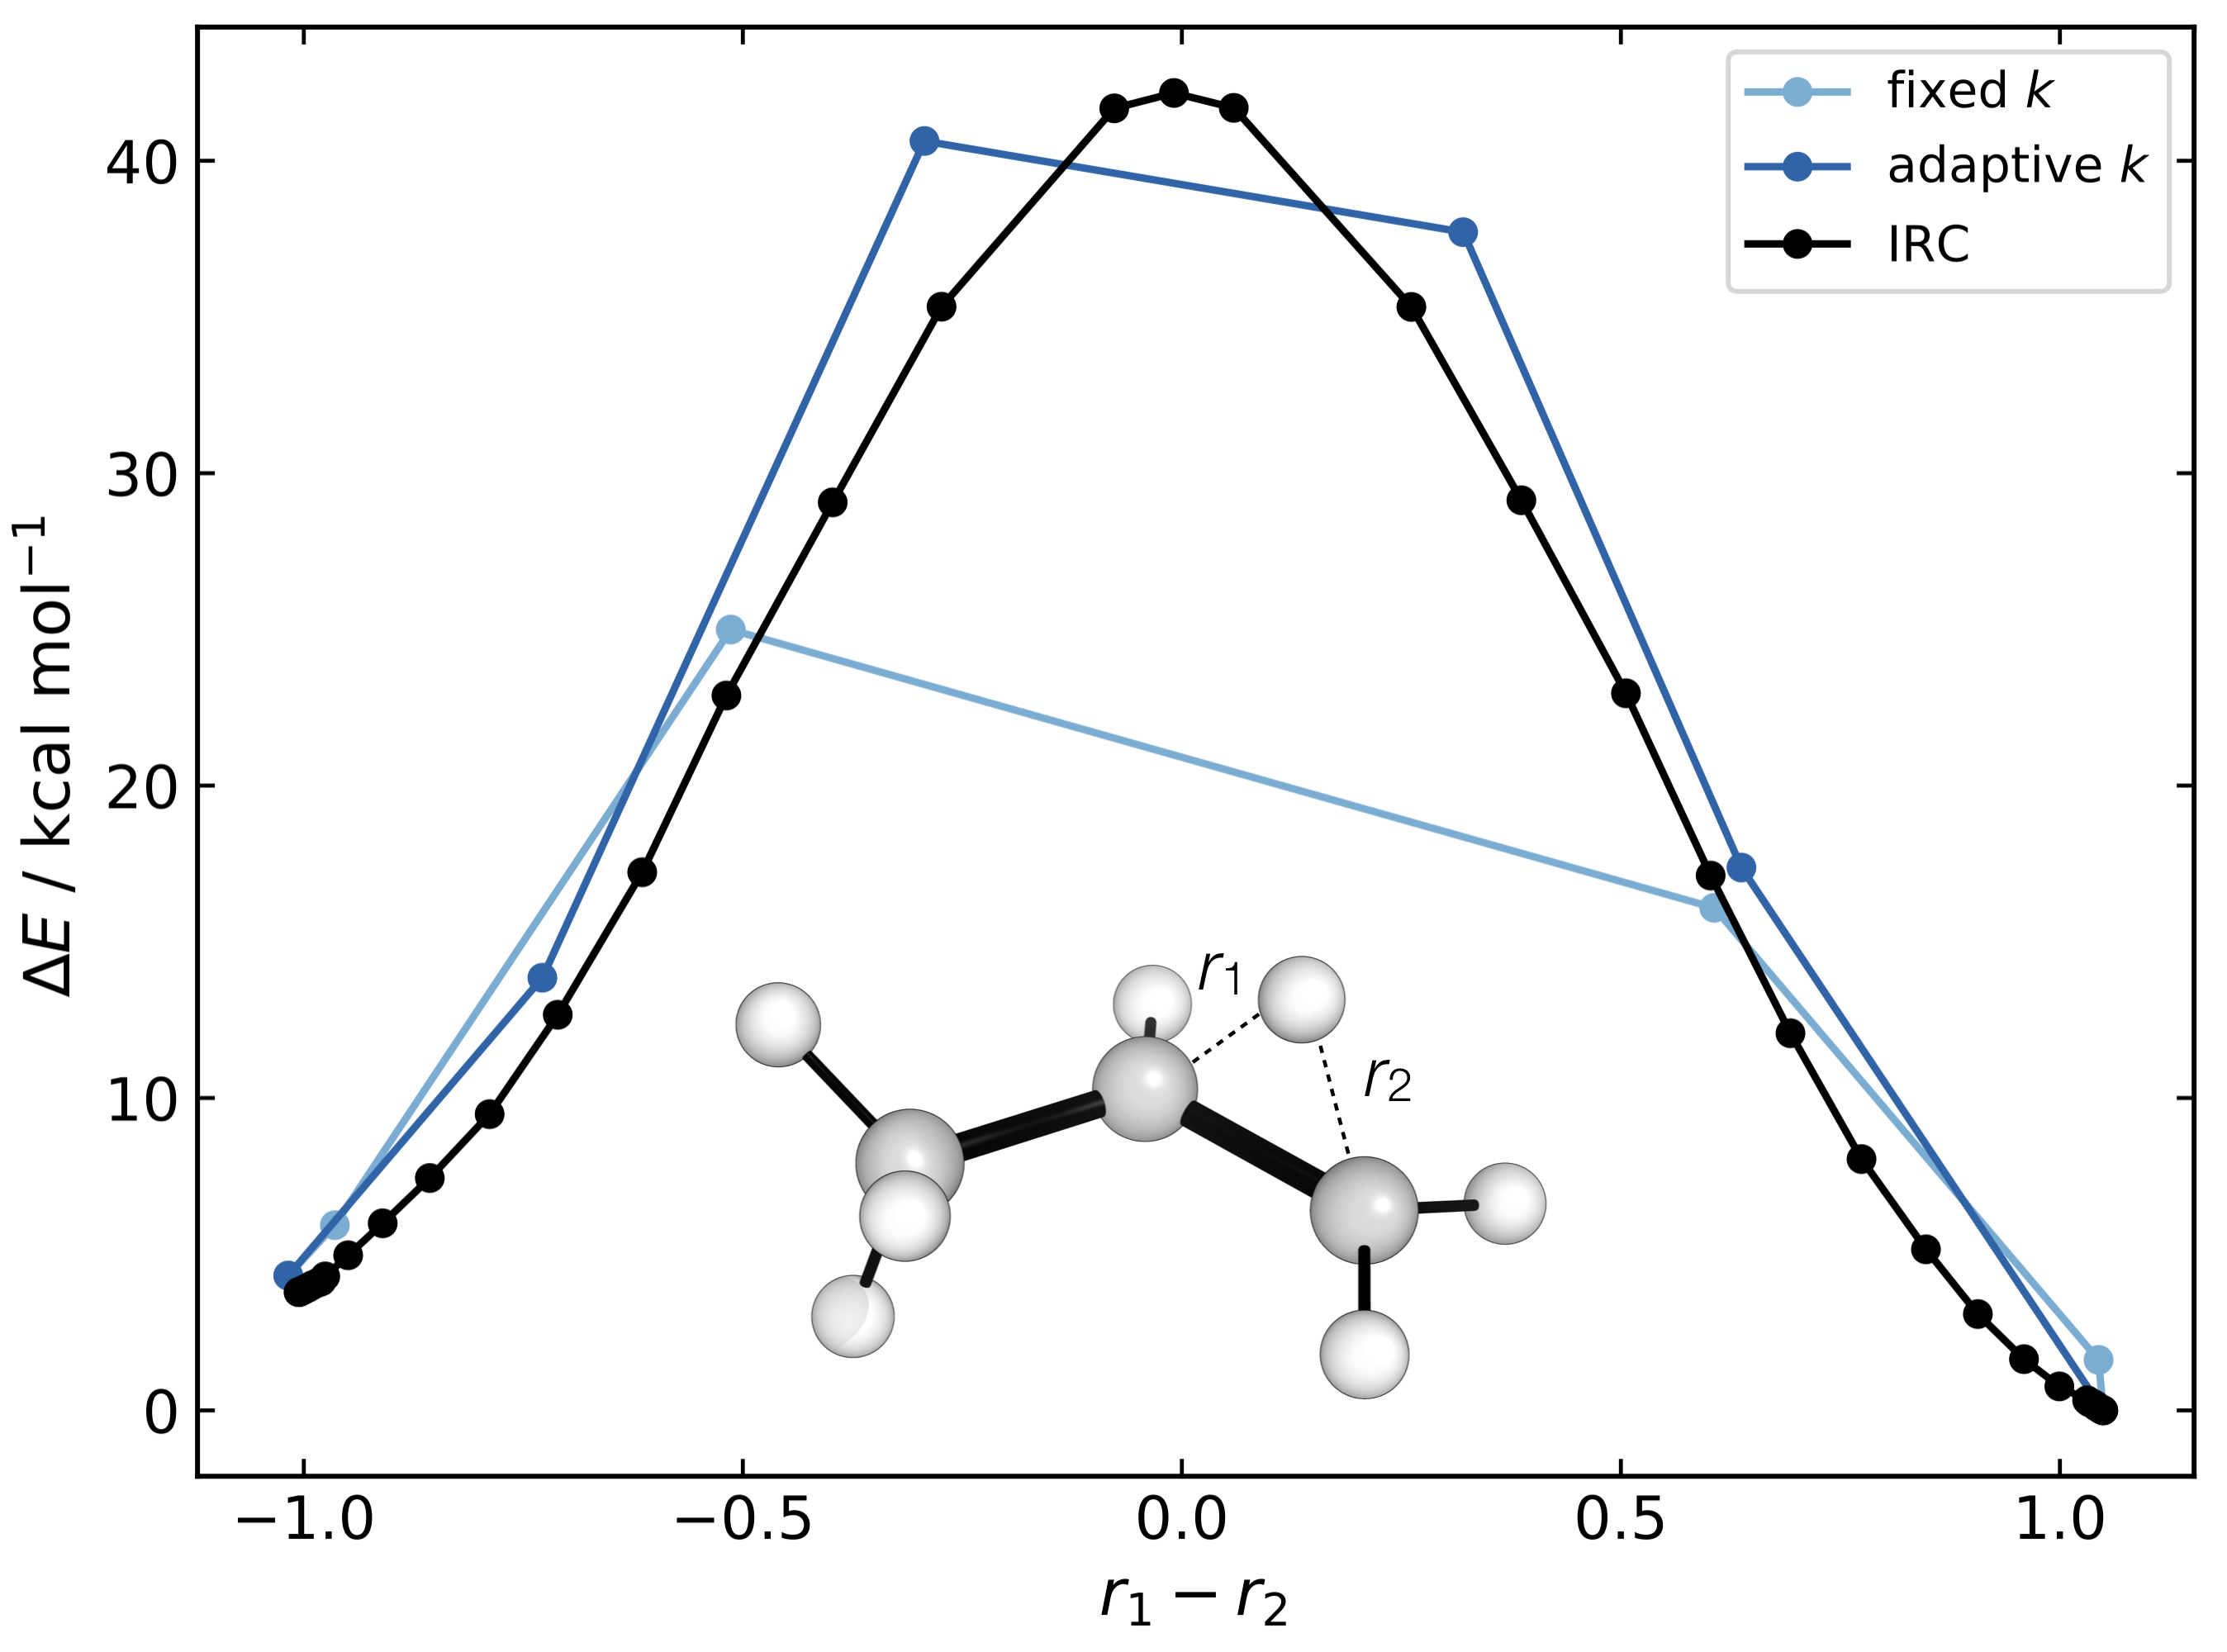
\includegraphics[width=10cm]{5/further/figs/fig1/fig1.png}
	\vspace{0.4cm}
	\hrule
	\caption{Comparison of approximate minimum energy pathways for the H-shift in a terminal propyl radical at the PBE0-D3BJ/def2-SVP level of theory. NEB paths in blue $k = 0.1$ Ha \AA$^{-1}$, fixed or adaptive according to Eq. \eqref{equation::neb_adaptive_k} and the reference IRC in black.}
	\label{fig::ade_further_1}
\end{figure}


While searching for an improved method to generate reaction paths upon which NEB relaxation may be performed, an algorithm was developed for traversing a reasonable initial pathway. Motivated by steepest-decent minimisation where the direction is defined by the gradient of the surface an `adaptive' path may be defined using gradient dependent constraints. The initial constraints for the first point are,
\begin{equation}
	r_b^{(1)} = r_b^{(0)} + \sgn(r_b^\text{final} - r_b^{(0)})\Delta r_\text{init}
\end{equation}
for an active bond $b$, where the superscript denotes the current step. $\Delta r_\text{init}$ is an initial step size, e.g. 0.2 \AA. Constraints for subsequent steps are then given by,
\begin{equation}
	r_b^{(k)} = r_b^{(k-1)} + \sgn(r_b^\text{final} - r_b^{(0)})\Delta r_b^{(k-1)}
\end{equation}

\begin{equation}
	\Delta r_b^{(k)} = 
	\begin{cases}
		\Delta r_\text{max} \quad &\text{if } \sgn(r_b^\text{final} - r_b^{(0)}) \nabla E_{j} \cdot \boldsymbol{r}_{ij} > 0 \\
		\Delta r_\text{m}\exp\left[-\left({\nabla E_{j}^{(k)} \cdot \boldsymbol{r}_{ij}}/{g} \right)^2\right] + \Delta r_\text{min} \quad &\text{otherwise}
	\end{cases}
\end{equation}
where $\Delta r_\text{m} = \Delta r_\text{max} - \Delta r_\text{min}$, $E$ the total potential energy (in the absence of any harmonic constraints) and $g$ a parameter to control the interpolation between $\Delta r_\text{max}$ and $\Delta r_\text{min}$ e.g. 0.05 Ha Å$^{-1}$. Atom indices $i, j$ form part of the bond indexed by $b$ with $j$ being an atom not being substituted. In the case that neither $i$ nor $j$ are being substituted the gradient is taken as an average over $i$ and $j$.

This approach generates a parameter dependent but remarkably accurate way of traversing close to a MEP with no \emph{a priori} knowledge. For the standard model London{\textendash}Eyring{\textendash}Polanyi {\textendash}Sato (LEPS) analytic 2D PES (see ref. \cite{MartinGondre2010} for a review and definition) a judicious choice of parameters can afford an excellent path (\figurename{ \ref{fig::ade_further_2}}).

Motivated by this accuracy a more complex, true chemical reaction path was traversed using the same method with parameters $\Delta r_\text{max} = 0.3$ \AA$\;$and $g = 0.05$ Ha \AA$^{-1}$. Specifically, for the fluoride + methyl chloride reaction employing a small minimum step size, a point within 0.1 \AA$\;$of the true TS is traversed, which is a good TS guess (i.e. transition state optimisation is successful in just a few geometry optimisation steps).


\begin{figure}[h!]
	\vspace{0.4cm}
	\centering
	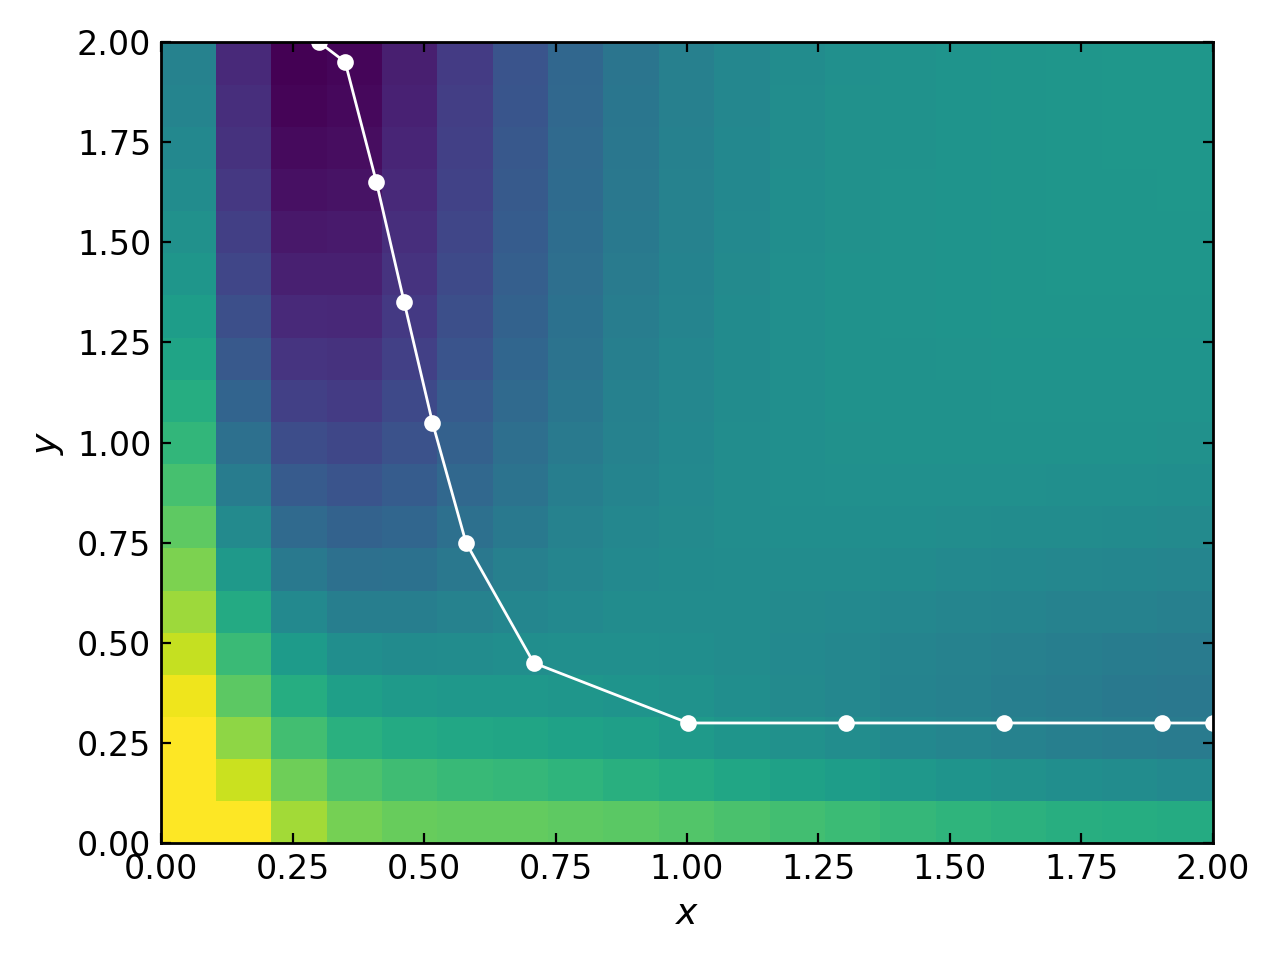
\includegraphics[width=11cm]{5/further/figs/fig2/fig2.png}
	\vspace{0.2cm}
	\hrule
	\caption{LEPS potential ($a = 0.05;
		b = 0.8;
		c = 0.0;
		r_0 = 0.742;
		\alpha = 1.942$) overlaid with an adaptive path, with parameters
		$\Delta r_\text{min} = 0.05, \Delta r_\text{max} = 0.3, g = 50$.}
	\label{fig::ade_further_2}
\end{figure}



\begin{figure}[h!]
	\vspace{0.4cm}
	\centering
	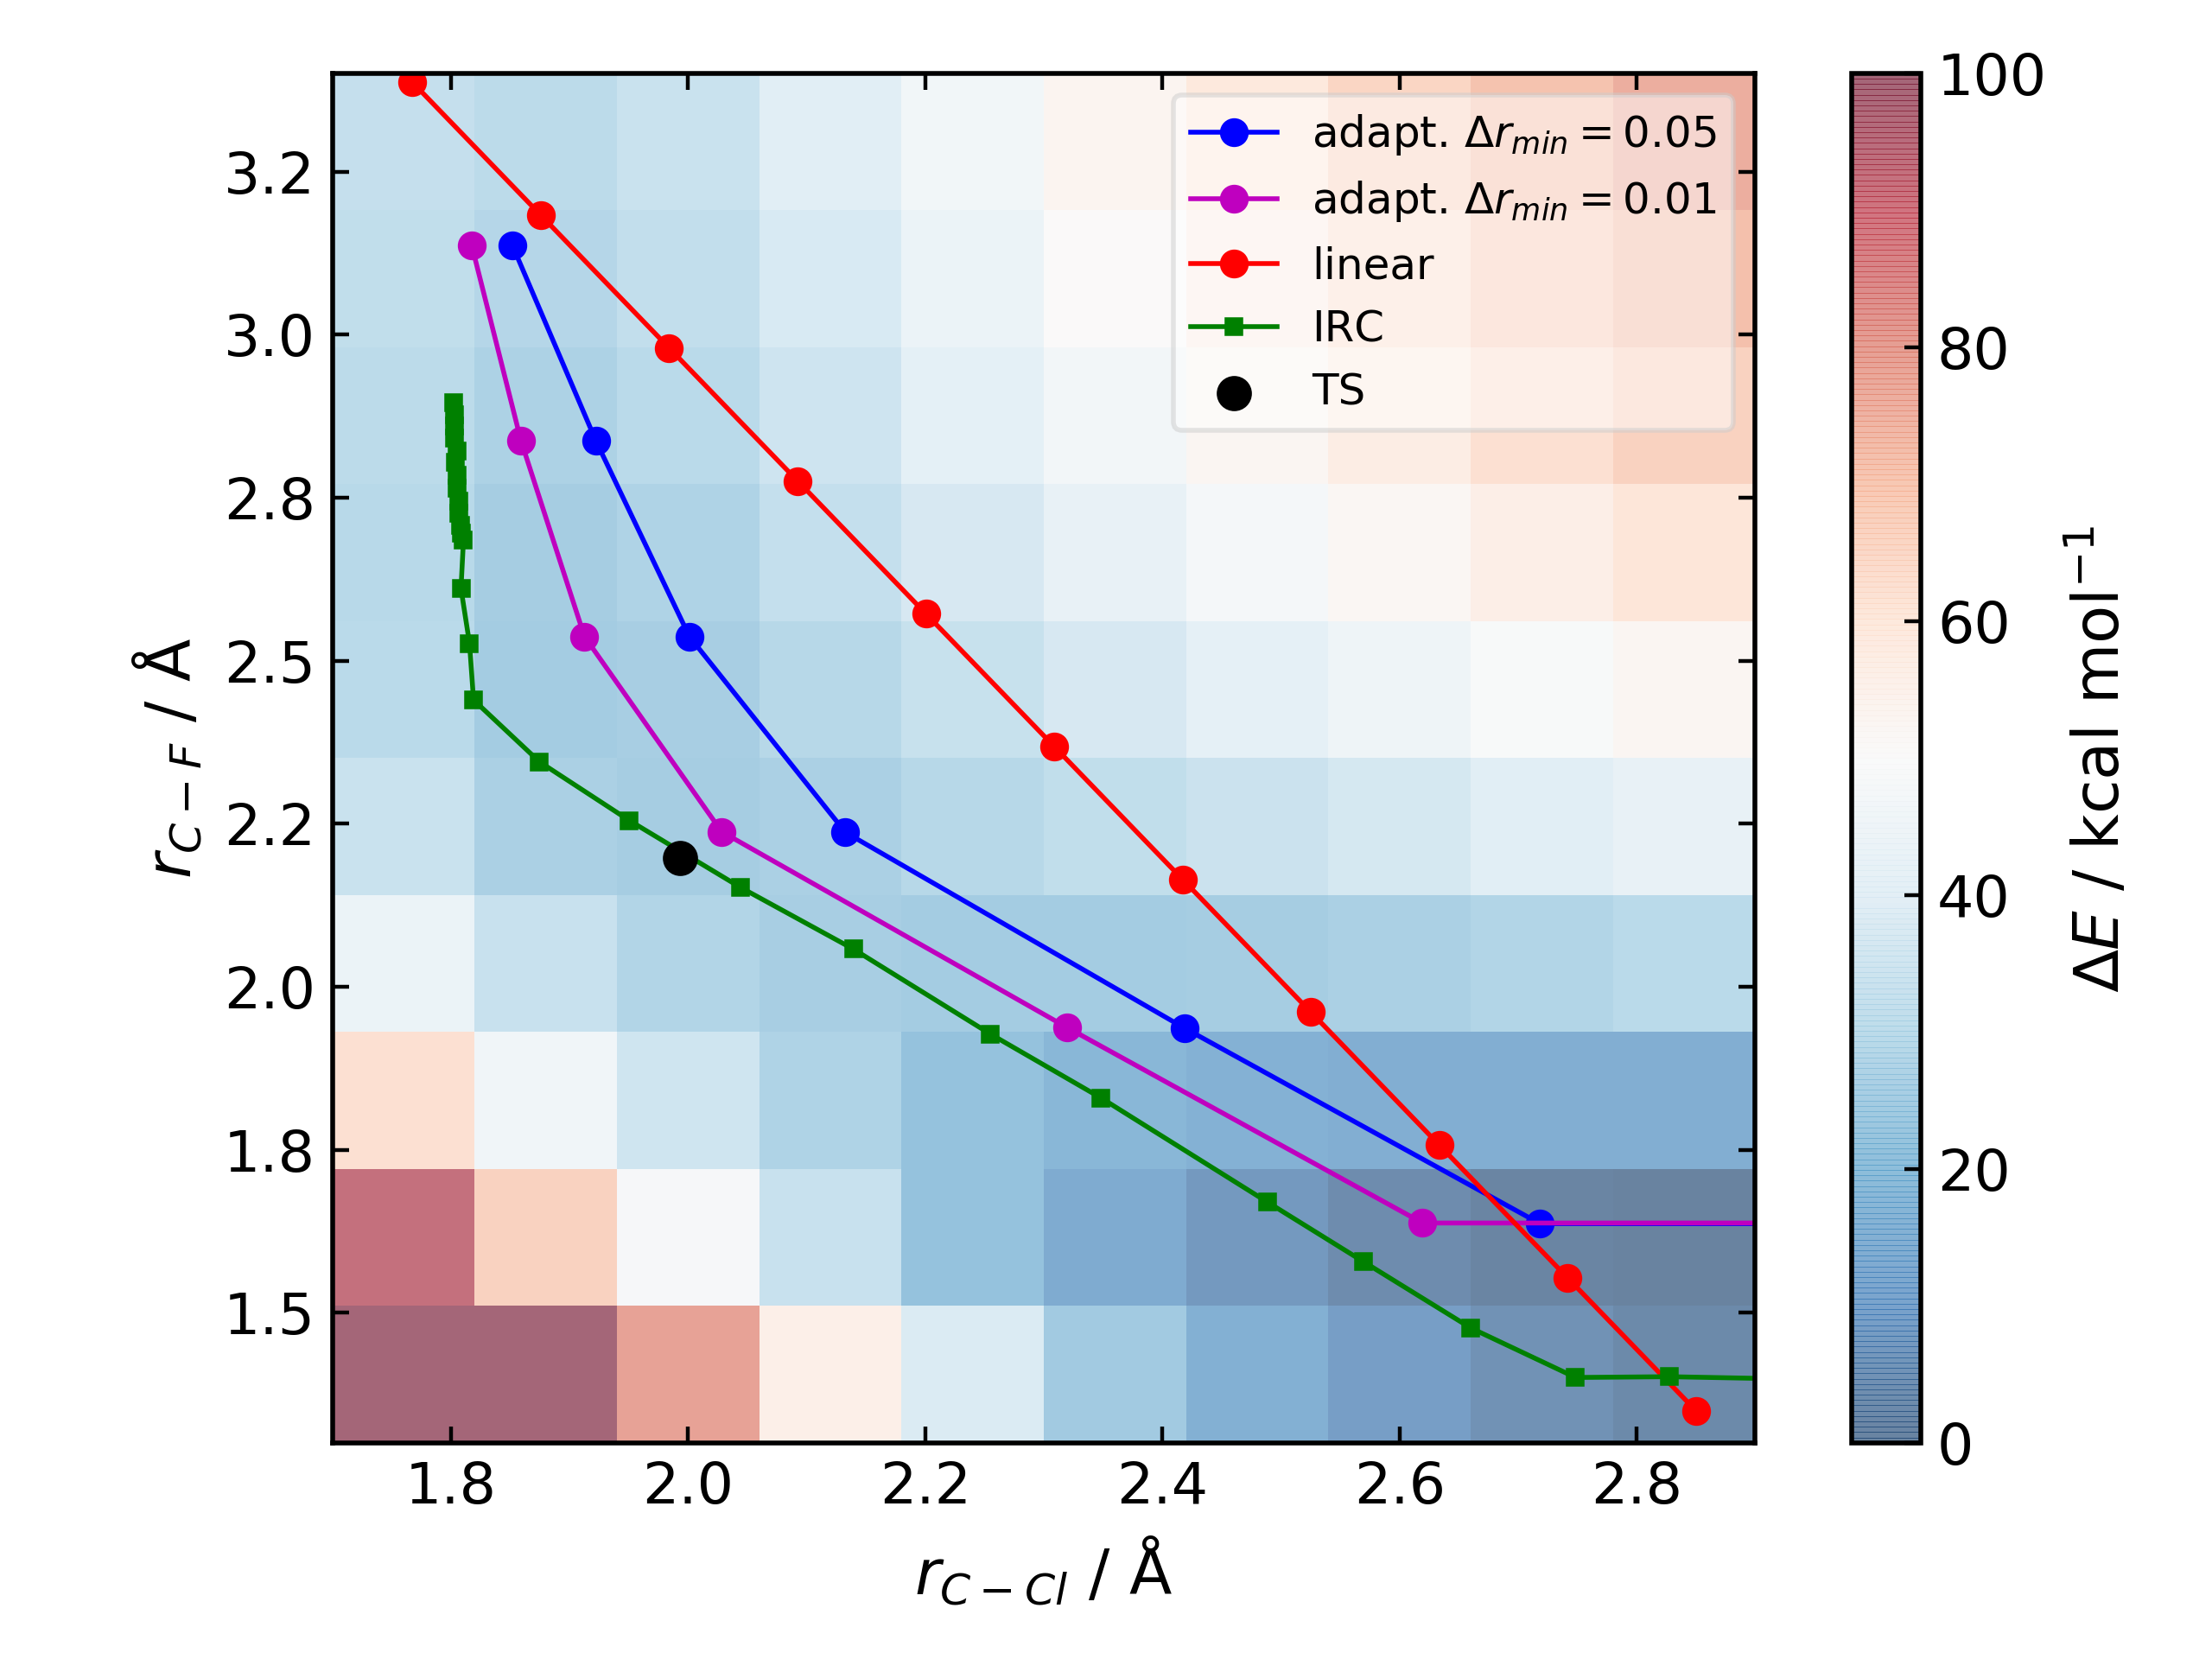
\includegraphics[width=12cm]{5/further/figs/fig3/fig3.png}
	\vspace{0.2cm}
	\hrule
	\caption{Relaxed 2D PES calculated at PBE0-D3BJ/ma-def2-SVP/CPCM(water) overlaid with adaptive paths the IRC and the true (optimised) TS highlighted.}
	\label{fig::ade_further_3}
\end{figure}


Further testing of this method suggests a significant performance benefit, for a set of small ($< 20$ atoms) organic reactions adapted from ref. \cite{Vaucher2018} (\figurename{ \ref{fig::ade_further_4}}) and small organometallic reactions\cite{autodE} (\figurename{ \ref{fig::ade_further_5}}) a guess TS is generated in $\sim 10$ minutes on 8 CPU cores in each case.

\begin{figure}[h!]
	\vspace{0.4cm}
	\centering
	
\includegraphics[width=15cm]{5/further/figs/fig4/fig4.png}
	\vspace{0.4cm}
	\hrule
	\caption{Small organic reactions.}
	\label{fig::ade_further_4}
\end{figure}

\begin{figure}[h!]
	\vspace{0.4cm}
	\centering
	
\includegraphics[width=15cm]{5/further/figs/fig5/fig5.png}
	\vspace{0.4cm}
	\hrule
	\caption{Small organometallic reactions. Explicitly defined valencies are required for accurate SMILES strings}
	\label{fig::ade_further_5} 
\end{figure}

In particular, for Diels-Alder reactions the performance increase over previously employed 2D relaxed PES scans is significant, as only a single coordinate is traversed resulting in at least a $10 \times$ speed-up. For this reason the adaptive path algorithm is now the default in \ade for all $(x, y)$ transformations (where $x$ bonds form and $y$ bonds break).


\subsection{Molecule Building}

Converting a SMILES string into a 3D geometry was achieved within \ade using RDKit\cite{Landrum2019} for organic molecules and using a SMILES parser and a randomise+relax algorithm on all atoms for metal complexes. This approach, however, comes with two drawbacks: (1) cyclic organic molecules containing \emph{trans} ($E$) double bonds are (as of RDKit v. 2020) generated as their \emph{cis} ($Z$) analogues and (2) randomising all atoms does not respect any stereochemistry defined in the SMILES string (point tetrahedral or $E$/$Z$).

To rectify these limitations a completely new (Open)SMILES parser was developed that is fast, well tested and extensible. From this, 3D geometries are built by:

\begin{enumerate}
	\item Converting all implicit hydrogen atoms defined in the SMILES string to explicit atoms (e.g. `CC' refers to a ethane molecule).
	\item Setting the atom types with templated vacant sites, for example a tri-coordinate atom is assigned a trigonal template unless it is a group 15 element in which case a trigonal-pyramidal geometry is defined. 
	\item For each atom in turn:
	\begin{enumerate}
		\item Translate the atom to the origin if it's the first to be added, or a vacant site on an already-translated atom.
		\item Rotate the empty sites on the atom such that one is coincident with the neighbouring atom.
	\end{enumerate}
\end{enumerate}

While simple, this approach is remarkably efficient at generating linear molecules, with an execution time generally $<100$ milliseconds. There are, of course, special cases that require some care. For example, double bonds with a defined $E/Z$ stereochemistry require the dihedral angle across the double bond to be adjusted appropriately. Rings and particularly fused rings are challenging to build using this approach, as added atoms can no longer be chosen to minimise the repulsion with the rest of the structure. Once ring atoms have been added sequentially the dihedral angles are adjusted to minimise,
\begin{equation}
	V = k(r-r_\text{avg})^2 + \sum_{i>j} {c_{ij}}/{r_{ij}^n}
\end{equation}
where $n$ is a positive integer and average distances $r_\text{avg}$ are taken from the CCDC. This `closes' the ring while maintaining a small steric repulsion. 

For a flat aromatic ring (e.g. phenyl) then the three dihedrals must be simply be zeroed. In a saturated or semi-saturated ring, however, many dihedrals must be minimised on as to close the ring. This is achieved using a stochastic global steepest-decent minimisation where random points in the space are selected.\footnote{Note an improved semi-stochastic algorithm by maximising the distance between the starting points in the $n$-dimensional space for $n$ dihedrals is under development.} Further complications arise when small rings ($< 5$-membered) or metallocycles are closed, as rotating dihedrals is no longer sufficient to adequately close a ring. In these contexts, either the bond angles within the ring are adjusted, or the whole ring minimised with a repulsion+bonded (RB) potential, as previously used to generate the whole structure.

\subsection{Future Development}

Currently, \ade provides access to reaction profiles for a wide range of reactions. However, some limitations remain that encourage further developments.Currently a maximum of four bonds can be been broken and formed in a a single step and the performance limited by the inaccuracy of `low-level’ electronic structure methods. Addressing these limitations will be the subject of future development, with the current focus on the following aspects:
 
\begin{itemize}
	\item Improved load balancing in conformer optimisation. Currently, each conformer optimisation or single-point energy evaluation is performed in serial. While this approach is close to optimal for calculations run on $\lesssim 8$ CPU cores, for which most electronic structure codes parallelise almost linearly up to, it is not for \ade calculations performed on more cores. A context-aware and dynamic multiprocessing approach therefore would be beneficial to reduce the total wall time.
	
	\item Consistent thermochemical calculations. Currently, \ade uses thermochemical data calculated by the electronic structure codes and is therefore inconsistent. Hessian extraction and diagonalisation to calculate frequencies thus enthalpy/entropy/free energies would provide a consistent framework.
	
	\item Implementation of minima and transition state optimisers. Currently, optimisations are performed using electronic structure codes, which means (1) Atomic Simulation Environment (ASE\cite{ASE2017})-wrapped codes cannot be used for efficient optimisations, as ASE optimisation are in Cartesian coordinates; (2) convergence criteria cannot be defined explicitly and (3) optimisations can crash irrevocably in both ORCA and Gaussian.\footnote{For example, when an angle approaches ${180}^{\circ}$ the calculation fails in Gaussian09, which is handled in \ade but requires a recursive fix, which may fail after a few attempts. On the other hand ORCA does not stop when the internal$\rightarrow$Cartesian back transformation fails, but enters a high-energy region of phase space.} Due to (2), an \emph{autodE}-based optimisation could afford faster path searches by employing loose convergence criteria for regions not close to the TS. Implementing minimisers would also enable greater functionality with newly emerging machine learned potentials (MLPs).
	
	\item Implementation of wrappers for other electronic structure packages e.g. TurboMole and PSI4. Adding these methods will enhance the flexibility and usability of \emph{autodE}.
	
	\item Improved conformer enumeration using an exhaustive algorithm. Currently, conformer generation is performed with RDKit for organic molecules and adding random displacements then minimising for organometallic species. However, for small and/or rigid molecules complete sampling of the conformational space may be possible and will provide the global minimum.
	
\end{itemize}

I expect most or all of these to be included with version 1.1, which will be released at some point in 2021, further enhancing the accuracy and speed of \emph{autodE}.


\clearpage
\end{document}
